\documentclass[tikz,border=12pt]{standalone}
\usepackage[T1]{fontenc}
\usepackage{mathpazo}
\usepackage{amsmath,amssymb}
\usetikzlibrary{arrows.meta, calc}

\definecolor{stblue}{HTML}{7B97AD}
\definecolor{rwgold}{HTML}{B8995E}
\definecolor{sage}{HTML}{7A9A7E}
\definecolor{dkbrown}{HTML}{3D3530}
\definecolor{wmgray}{HTML}{7B7067}
\definecolor{cream}{HTML}{F9F6F0}
\definecolor{border}{HTML}{D4C9B8}
\definecolor{terracotta}{HTML}{C47A6A}
\definecolor{lavender}{HTML}{907EA0}

\begin{document}
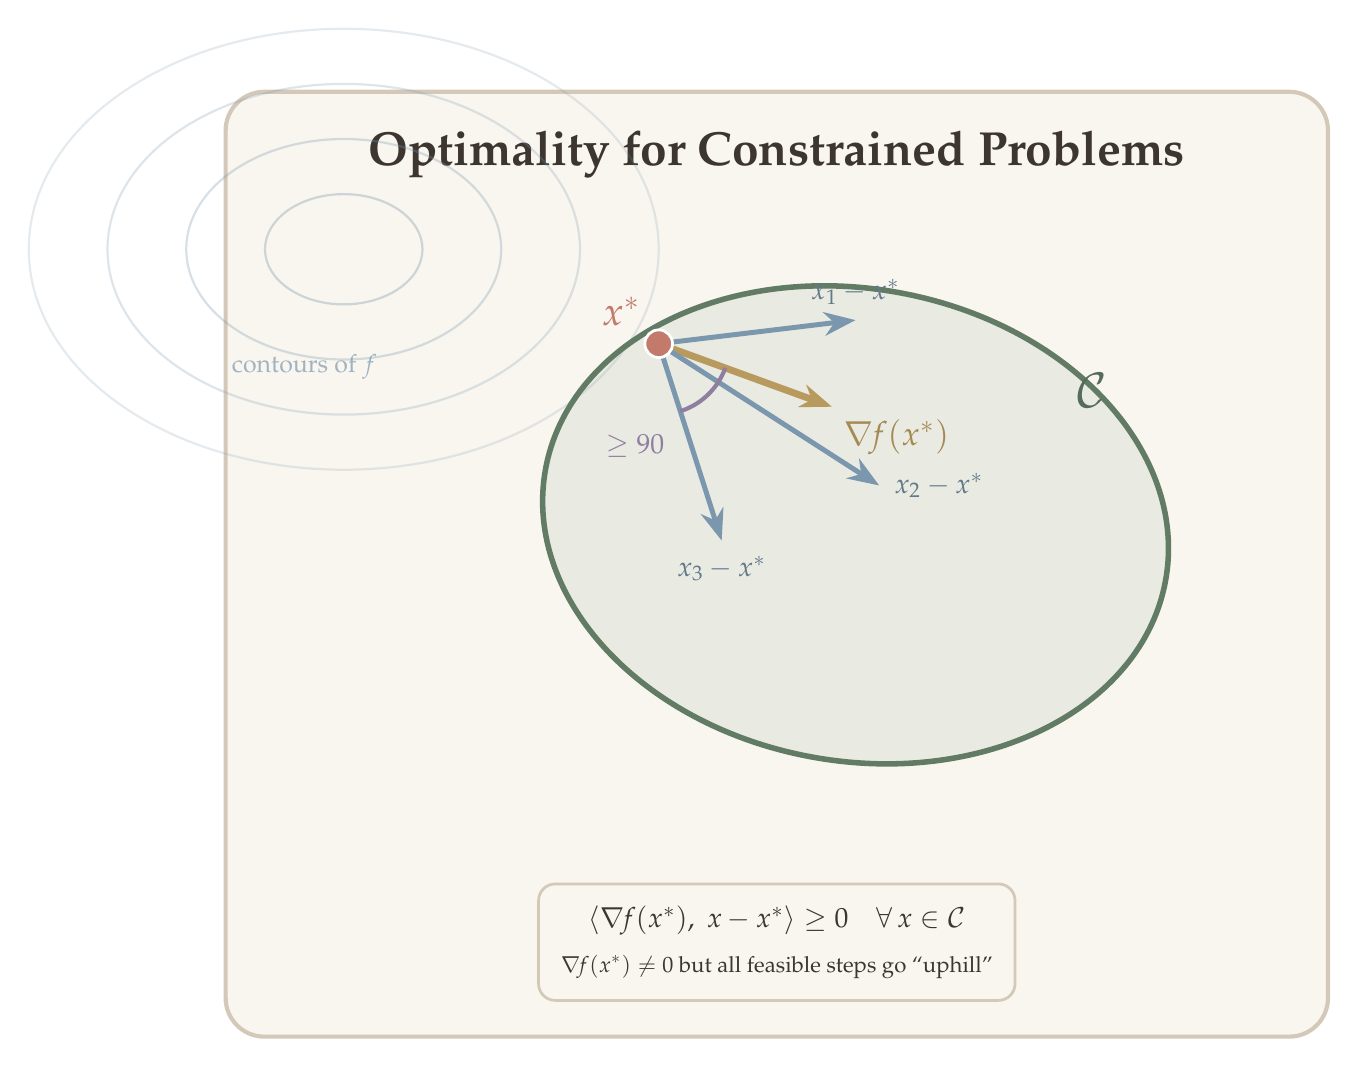
\begin{tikzpicture}[>={Stealth[length=4mm, width=3mm]}]

% Background
\fill[cream, rounded corners=14pt] (-1.5,-3.0) rectangle (12.5,9.0);
\draw[border, line width=1.5pt, rounded corners=14pt] (-1.5,-3.0) rectangle (12.5,9.0);

% Title
\node[text=dkbrown, font=\LARGE\bfseries] at (5.5,8.2)
  {Optimality for Constrained Problems};

% Contour lines of f (centered outside C, upper-left)
\foreach \r/\op in {1.0/0.35, 2.0/0.30, 3.0/0.25, 4.0/0.20} {
  \draw[stblue, line width=0.8pt, opacity=\op]
    (0.0,7.0) ellipse ({\r*1.0} and {\r*0.7});
}
\node[text=stblue, font=\small, opacity=0.7] at (-0.5,5.5) {contours of $f$};

% Convex set C (tilted ellipse)
\begin{scope}[rotate around={-10:(6.5,3.5)}]
  \fill[sage, opacity=0.12] (6.5,3.5) ellipse (4.0cm and 3.0cm);
  \draw[sage!80!black, line width=2pt] (6.5,3.5) ellipse (4.0cm and 3.0cm);
\end{scope}

% Label C
\node[text=sage!70!black, font=\LARGE\bfseries] at (9.5,5.2) {$\mathcal{C}$};

% Constrained optimum x* (on boundary, upper-left region of C)
\coordinate (xstar) at (4.0,5.8);

% Gradient at x* (points away from unconstrained optimum, into C)
\draw[rwgold, line width=2.5pt, ->]
  (xstar) -- ($(xstar)+(2.2,-0.8)$);
\node[text=rwgold!90!black, font=\large\bfseries, below right=1pt]
  at ($(xstar)+(2.2,-0.8)$) {$\nabla\!f(x^*)$};

% Feasible directions from x*
\coordinate (d1) at ($(xstar)+(2.5,0.3)$);
\coordinate (d2) at ($(xstar)+(2.8,-1.8)$);
\coordinate (d3) at ($(xstar)+(0.8,-2.5)$);

\draw[stblue, line width=1.8pt, ->] (xstar) -- (d1);
\node[text=stblue!80!black, font=\normalsize, above=2pt] at (d1) {$x_1 - x^*$};

\draw[stblue, line width=1.8pt, ->] (xstar) -- (d2);
\node[text=stblue!80!black, font=\normalsize, right=2pt] at (d2) {$x_2 - x^*$};

\draw[stblue, line width=1.8pt, ->] (xstar) -- (d3);
\node[text=stblue!80!black, font=\normalsize, below=2pt] at (d3) {$x_3 - x^*$};

% Obtuse angle arc between gradient direction and feasible directions
\pgfmathanglebetweenpoints{\pgfpointanchor{xstar}{center}}{\pgfpointxy{6.2}{5.0}}
\let\angGrad\pgfmathresult
\pgfmathanglebetweenpoints{\pgfpointanchor{xstar}{center}}{\pgfpointanchor{d3}{center}}
\let\angD\pgfmathresult

\draw[lavender, line width=1.5pt]
  ($(xstar)+({\angD}:0.9cm)$) arc[start angle=\angD, end angle=\angGrad, radius=0.9cm];
\node[text=lavender, font=\normalsize\bfseries] at ($(xstar)+(-0.3,-1.3)$) {$\geq 90°$};

% x* point (on top)
\fill[terracotta] (xstar) circle (5pt);
\draw[white, line width=1pt] (xstar) circle (5pt);
\node[text=terracotta, font=\Large\bfseries, above left=3pt] at (xstar) {$x^*$};

% --- Annotation box (self-contained node) ---
\node[text=dkbrown, font=\normalsize,
      fill=cream, inner sep=8pt, align=center,
      draw=border, line width=1pt, rounded corners=6pt]
  at (5.5,-1.8)
  {$\langle \nabla\!f(x^*),\; x - x^* \rangle \geq 0 \quad \forall\, x \in \mathcal{C}$\\[4pt]
   \footnotesize $\nabla\!f(x^*) \neq 0$ but all feasible steps go ``uphill''};

\end{tikzpicture}
\end{document}
